% Classe para teses e dissertações no IFSC - USP
%
% 
% autor: Thiago S. Mosqueiro
% e-mail contato: thiago -dot- mosqueiro (at) ursa.ifsc.usp.br
% Site com informações sobre a classe:
% http://thmosqueiro.vandroiy.com/ifsc-latex/
%
% Se você estiver chamando latex + dvi2ps + ps2pdf, sua folha sairá em letter (não a4)
% a menos que você: (i) adicione -sPAPERSIZE=a4 à chamada do ps2pdf ou (ii) configure
% como saída padrão o papel a4.
%
%
% Bom uso de LaTeX a todos!!
%


\documentclass[a4paper, espaco=emeio, dvips, plainheader, twoside, openright, final, normalfigtabnum, tocpage=plain, titulodireita]{ifsc}
  
  
  \usepackage{additionals}

% A opção linktocpage é muito importante para poder fazer com que TOC tenha
% quebra de linhas!!!
  \usepackage[colorlinks, hyperindex, breaklinks]{hyperref}
  \hypersetup
  {
    pdftitle = {T\'{\i}tulo da sua tese},
    pdfauthor = {Nome do autor},
    pdfsubject = {Assunto da tese},
    pdfkeywords = {Palavras-chave},
    pdfcreator = {Como você compilou o tex?},
    linkbordercolor = {1 0 0},
    pdftoolbar = true,
    pdfmenubar = true,
    colorlinks = false,
    citecolor=black,
    linkcolor=black,
    urlcolor=black,
  }

  \makeindex
  
  \def\@cite#1#2{({#1\if@tempswa:#2\fi})}
  
  \setlength{\footnotemargin}{0in}


  % Pasta onde voce vai deixar suas imagens
  \graphicspath{{figuras/}}

 % Caso seja a versão corrigida, descomente abaixo.
 % \renewcommand{\IFSCversao}{Vers\~ao Corrigida\\ (versão original disponível na Unidade que aloja o Programa)}

  \usepackage{tikz}
  
  % Neste arquivo você pode inserir suas definições (veja exemplo)
  % Arquivo com atalhos

% Definindo um ket
\newcommand{\ket}[1]{\left| #1 \right\rangle}

  \begin{document}


    \universidade{Universidade de S�o Paulo \\ Instituto de F�sica de S�o Carlos}

\autor{Gabriel Luchini}

\titulo{T\'{\i}tulo da sua tese}

\orientador{Prof. Dr. Nome do Seu Orientador}

\area{F�sica B�sica}

\comentario{Disserta��o apresentada ao Programa de P�s-Gradua��o em F�sica do Instituto de F�sica de S�o Carlos da Universidade de S�o Paulo, para obten��o do t�tulo de mestre em Ci�ncias.}

\instituicao{Grupo de F�sica Te�rica \par Departamento de Ci�ncias dos Materiais \par Instituto de F�sica de S�o Carlos - Universidade de S�o Paulo}

\local{S�o Carlos}

\data{2011}

\capa

\folhaderosto

\begin{center}
  {\scshape \ttfamily AUTORIZO A REPRODU��O E DIVULGA��O TOTAL OU PARCIAL DESTE TRABALHO, POR QUALQUER MEIO CONVENCIONAL OU ELETR�NICO, PARA FINS DE ESTUDO E PESQUISA, DESDE QUE CITADA A FONTE.}
  
  \vfill
  
  \begin{center}
    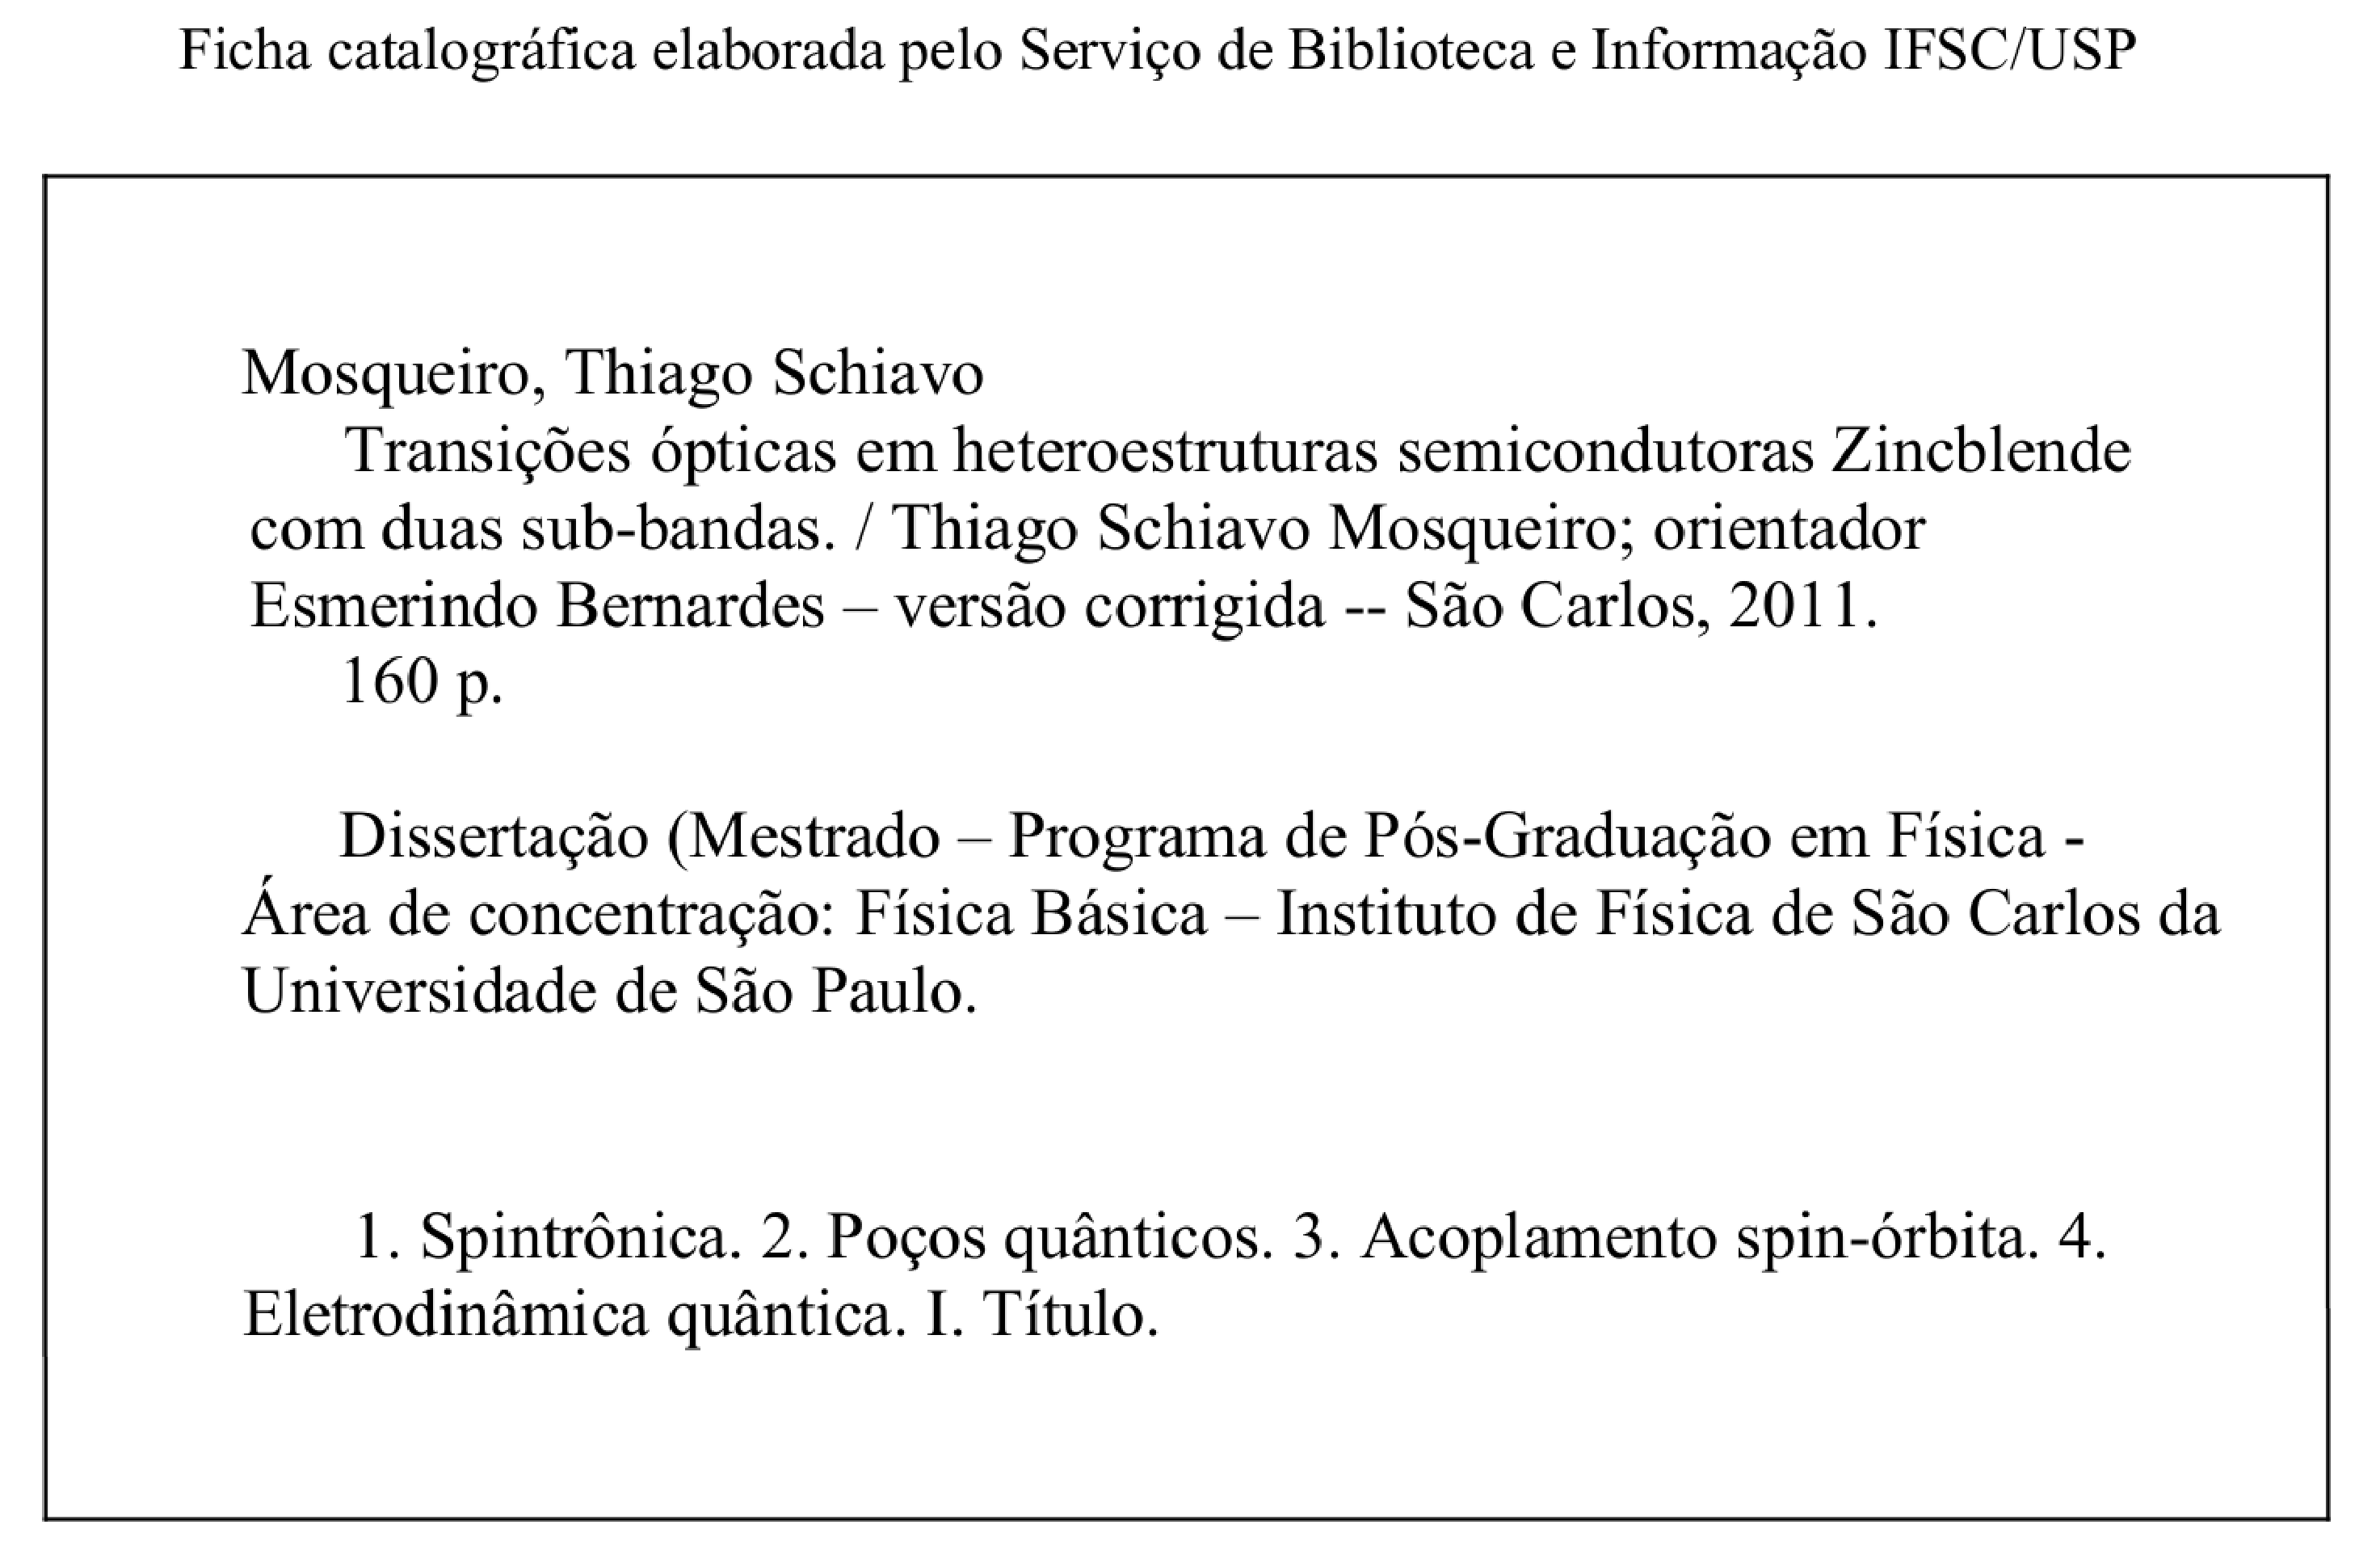
\includegraphics[scale = 0.28]{fichacatalografica}
  \end{center}
\end{center}


% \begin{folhadeaprovacao}
% Disserta��o apresentada ao Programa de P�s-Gradua��o em F�sica do Instituto de F�sica de S�o Carlos da Universidade de S�o Paulo, para obten��o do t�tulo de mestre em Ci�ncias.
% 
% \assinatura{Prof. Dr. Esmerindo de Sousa Bernardes\\ Orientador}  
% \assinatura{Prof. Dr. Iouri Poussep\\ Instituto de F�sica de S�o Carlos -- Universidade de S�o Paulo}
% \assinatura{Prof. Dr. Marcel Novaes\\ Departamento de F�sica -- Universidade Federal de S�o Carlos}
% \end{folhadeaprovacao}

    \begin{agradecimentos}
Agradecimentos v�m aqui.

\end{agradecimentos}

\newpage

\phantom{11}
\vfill\vfill\vfill
\begin{flushright}
  \begin{minipage}{0.7\textwidth}
    \emph{Uma ep�grafe pode ser utilizada aqui. Ela pode ser longa, conter diversas partes, qualquer coisa. O LaTeX far� ficar bem posicionada.}
    \newline
    \newline
    \scriptsize{Refer�ncia da sua ep�grafe.}
  \end{minipage}
\end{flushright}

    \chapter*{RESUMO}

\begin{citacaotese}
	SOBRENOME, T. S. \textit{T�tulo da tese entra aqui}. 2011. 160 p. Disserta��o de Mestrado -- Instituto de F�sica de S�o Carlos, Universidade de S�o Paulo, S�o Carlos, 2011.
\end{citacaotese}

\begin{resumo}
	Lorem ipsum dolor sit amet, consectetur adipiscing elit. Suspendisse quis arcu nisl, eu venenatis sapien. Maecenas consectetur leo nibh. Cras vitae nisi quis lacus hendrerit sagittis. Sed nec libero elit. Aenean gravida, libero a aliquet lacinia, erat odio ornare neque, ut pretium turpis libero sit amet sapien. Fusce lacinia viverra massa, et pretium dolor blandit quis. Curabitur ultricies lacus vitae felis blandit consequat. Mauris mollis malesuada lacus, et suscipit magna pellentesque vel. Fusce at tincidunt mi. Integer dignissim est quis sapien laoreet tincidunt. Fusce egestas accumsan orci, et commodo tellus suscipit vel. Cras auctor ipsum ut purus rutrum vulputate. Pellentesque eget blandit turpis. Pellentesque in lacus sed justo vulputate porttitor. Donec tristique urna nec justo dictum consectetur. Etiam commodo molestie dictum. Curabitur mauris orci, lobortis ac vehicula et, ultrices vel mi. Aenean mollis erat a enim dapibus et convallis tortor ornare. Duis eleifend lectus ut nisi tincidunt et commodo ante adipiscing. Donec cursus felis eleifend lacus luctus porta. Aenean aliquam est et nisi gravida eget gravida velit ultrices. In quis semper urna. Maecenas sed augue et nibh lacinia ultrices. Aliquam viverra, augue a pellentesque blandit, libero lorem auctor lorem, nec luctus lectus nunc eget orci. Nulla sit amet neque in tortor placerat varius sed non augue. Cras elementum dignissim arcu, at vehicula metus malesuada rhoncus. Vestibulum sit amet vestibulum risus. Proin eros velit, molestie ut interdum commodo, hendrerit a ante. Aliquam molestie risus condimentum dolor faucibus eget convallis neque congue. Maecenas viverra nisi id turpis consequat eu consectetur diam blandit. Ut facilisis, erat sit amet sagittis gravida, mi dui facilisis justo, tristique consectetur libero nibh vitae arcu. Vestibulum ultricies, tellus eu facilisis porta, felis nulla semper elit, eget semper magna arcu et neque. Donec sed lorem purus, sit amet bibendum justo. Fusce at tincidunt mi. Integer dignissim est quis sapien laoreet tincidunt. Fusce egestas accumsan orci, et commodo tellus suscipit vel. Cras auctor ipsum ut purus rutrum vulputate. Pellentesque eget blandit turpis. Pellentesque in lacus sed justo vulputate porttitor. Donec tristique urna nec justo dictum consectetur. Etiam commodo molestie dictum. Curabitur mauris orci, lobortis ac vehicula et, ultrices vel mi.
\end{resumo}

\begin{palavraschave}
	Spintr�nica. Po�os qu�nticos. Acoplamento spin-�rbita. Eletrodin�mica qu�ntica.
\end{palavraschave}

\chapter*{ABSTRACT}

\hspace{-0.9cm} MOSQUEIRO, T. S. \textit{Title of the Thesis Here}. 2011. 160 p. Disserta��o de Mestrado -- Instituto de F�sica de S�o Carlos, Universidade de S�o Paulo, S�o Carlos, 2011.

\begin{resumo}
	Lorem ipsum dolor sit amet, consectetur adipiscing elit. Suspendisse quis arcu nisl, eu venenatis sapien. Maecenas consectetur leo nibh. Cras vitae nisi quis lacus hendrerit sagittis. Sed nec libero elit. Aenean gravida, libero a aliquet lacinia, erat odio ornare neque, ut pretium turpis libero sit amet sapien. Fusce lacinia viverra massa, et pretium dolor blandit quis. Curabitur ultricies lacus vitae felis blandit consequat. Mauris mollis malesuada lacus, et suscipit magna pellentesque vel. Fusce at tincidunt mi. Integer dignissim est quis sapien laoreet tincidunt. Fusce egestas accumsan orci, et commodo tellus suscipit vel. Cras auctor ipsum ut purus rutrum vulputate. Pellentesque eget blandit turpis. Pellentesque in lacus sed justo vulputate porttitor. Donec tristique urna nec justo dictum consectetur. Etiam commodo molestie dictum. Curabitur mauris orci, lobortis ac vehicula et, ultrices vel mi. Aenean mollis erat a enim dapibus et convallis tortor ornare. Duis eleifend lectus ut nisi tincidunt et commodo ante adipiscing. Donec cursus felis eleifend lacus luctus porta. Aenean aliquam est et nisi gravida eget gravida velit ultrices. In quis semper urna. Maecenas sed augue et nibh lacinia ultrices. Aliquam viverra, augue a pellentesque blandit, libero lorem auctor lorem, nec luctus lectus nunc eget orci. Nulla sit amet neque in tortor placerat varius sed non augue. Cras elementum dignissim arcu, at vehicula metus malesuada rhoncus. Vestibulum sit amet vestibulum risus. Proin eros velit, molestie ut interdum commodo, hendrerit a ante. Aliquam molestie risus condimentum dolor faucibus eget convallis neque congue. Maecenas viverra nisi id turpis consequat eu consectetur diam blandit. Ut facilisis, erat sit amet sagittis gravida, mi dui facilisis justo, tristique consectetur libero nibh vitae arcu. Vestibulum ultricies, tellus eu facilisis porta, felis nulla semper elit, eget semper magna arcu et neque. Donec sed lorem purus, sit amet bibendum justo. Fusce at tincidunt mi. Integer dignissim est quis sapien laoreet tincidunt. Fusce egestas accumsan orci, et commodo tellus suscipit vel. Cras auctor ipsum ut purus rutrum vulputate. Pellentesque eget blandit turpis. Pellentesque in lacus sed justo vulputate porttitor. Donec tristique urna nec justo dictum consectetur. Etiam commodo molestie dictum. Curabitur mauris orci, lobortis ac vehicula et, ultrices vel mi.
\end{resumo}

\begin{keywords}
	Spintronics. Quantum well. Spin-orbit coupling. Quantum electrodynamics.
\end{keywords}

    \listoffigures
    \newpage

    \listoftables
    \newpage

    \tableofcontents
    \newpage

    \chapter{Introdu\c{c}\~ao}
\label{chap:intro}

\begin{epigrafe}
	A vigan\c{c}a nunca \'e plena, mata a alma e a envenena.
	
	\autorepigrafe{Don Ramon}
\end{epigrafe}

Este eh um exemplo de tese. \cite{bastard1988, myself1stschoolspintronicap21,Crutchfieldnp8172012}

Lorem ipsum dolor sit amet, consectetur adipiscing elit. Nunc vitae accumsan nisl. In aliquet, risus nec semper lacinia, neque augue gravida urna, non consectetur eros massa a ipsum. Praesent iaculis auctor nunc, non lobortis eros malesuada vitae. Vivamus arcu arcu, pulvinar eu rutrum in, gravida vel metus. Donec libero tellus, porttitor in consequat eget, varius quis turpis. Mauris hendrerit sagittis tellus, rutrum rutrum enim euismod vitae. Aliquam sit amet lorem metus. Maecenas neque elit, fringilla quis fringilla at, vulputate a felis. Phasellus facilisis magna dictum quam sodales vel imperdiet turpis sodales. Integer non metus ut arcu volutpat condimentum. Nunc turpis mi, adipiscing et fringilla ut, eleifend nec libero. Aenean molestie accumsan sapien, et egestas sapien varius ac.

Outra cita\c{c}\~ao\cite{PhysRevB.76.195439}

\section{Primeira se\c{c}\~ao da sua tese}

Mauris eu tellus metus. Donec placerat sagittis lorem, et rhoncus diam semper tempus. Aliquam mattis tellus et nulla dignissim non mattis augue fermentum. Nullam lobortis bibendum nulla ut condimentum. Sed sed turpis at magna lacinia semper id ac risus. Praesent bibendum risus ac nulla feugiat molestie. Morbi non gravida sem. In a tristique velit. In congue dolor enim, quis blandit nulla. Nulla bibendum tortor neque.

Proin vitae dolor non ipsum iaculis tempor. Nunc eget sapien nisi. Nullam lobortis urna purus. Curabitur sed eros dui, sed elementum felis. Donec vel erat ligula. Pellentesque in libero et nibh congue dapibus. In tristique nunc nec enim suscipit ultricies.

Sed nec aliquam mauris. Curabitur placerat, risus ac gravida bibendum, metus tortor aliquet eros, in vestibulum ipsum erat eu nibh. Aenean sit amet purus magna. Fusce euismod, ligula ac consequat tempus, sapien turpis tempor est, quis pulvinar enim risus eget massa. Nunc ornare, purus in pulvinar tempor, nunc dui hendrerit ipsum, condimentum consequat quam lorem id nisi. Cras feugiat neque sed eros vulputate fermentum rutrum felis aliquet. Nam mollis commodo volutpat. In a interdum mi. Aliquam a nisl risus. In sem turpis, bibendum et venenatis a, venenatis et urna.

Duis eleifend viverra neque, id auctor libero fermentum vitae. Proin eu nibh turpis, ac fringilla neque. Nam mattis commodo rhoncus. Donec elementum malesuada ultrices. Sed viverra, velit at elementum porttitor, erat nisl ultricies diam, ac eleifend ipsum lacus in sapien. Duis sit amet mi felis. Nunc dignissim nibh mauris. Nunc porttitor fringilla tristique. Cras vel risus in tellus tristique tempus. Nam eu eros erat. Praesent sed metus nisl, ac tempor lorem. Aenean at velit vitae ante feugiat laoreet ac eu risus.

Nulla facilisi. Suspendisse id massa eu nisi malesuada luctus. Morbi feugiat eros id magna tristique accumsan. Phasellus elementum nunc id est imperdiet ac congue justo molestie. Morbi lobortis gravida velit, nec varius turpis vestibulum nec. Donec nec nisi sit amet risus lobortis bibendum. Aliquam turpis sem, rutrum nec mattis non, facilisis sed tellus. Aenean ut risus neque. Sed mattis, tortor non ultrices convallis, purus erat condimentum libero, id tristique elit metus vitae tellus. Sed laoreet mauris nec lacus pretium facilisis. Donec sem ipsum, porta quis laoreet quis, adipiscing ac tellus. Duis vestibulum, lorem ac rutrum varius, urna orci pretium sem, non luctus dolor ipsum et tortor. Aenean et fringilla lectus. In vitae velit libero, malesuada posuere augue. Fusce nisi sem, lobortis non malesuada at, consectetur ac sapien. Cras eleifend fringilla neque, non interdum sapien interdum rhoncus.

%\begin{figure}
%	\centering
%	
\includegraphics[scale=0.5]{open_source.eps}
%	\caption{Integer cursus rhoncus sem, ut pretium felis porta vitae. Cras facilisis convallis urna vel laoreet. Integer adipiscing metus at sapien tempus ultricies blandit eros dapibus. Nulla convallis, nunc et porttitor varius, metus lorem facilisis libero, in pulvinar enim ipsum eget lorem. Aliquam erat volutpat. Donec accumsan lacinia tincidunt. Praesent ac congue ipsum.}
%	\label{fig:exemplo}
%\end{figure}

Aqui estamos chamando a figura \ref{fig:exemplo}, e aqui chamamos uma nota de rodap\'e\footnote{Nulla sit amet neque est. Integer mattis dictum vulputate. In porttitor imperdiet tortor a aliquet.}. Note que a nota de rodap\'e j\'a est\'a usando s\'{\i}mbolos, e a numera\c{c}\~ao da figura leva em conta o cap\'{\i}tulo. Isso pode ser facilmente modificado!

Aliquam et est odio\footnote{Vestibulum iaculis tortor et leo faucibus pellentesque lacinia elit consequat.}. Cum sociis natoque penatibus et magnis dis parturient montes, nascetur ridiculus mus. Curabitur enim eros, congue et interdum id, posuere ut sapien. Mauris libero nunc, pharetra eget vestibulum vel, pellentesque id justo. Curabitur eleifend, arcu quis posuere egestas, risus purus rhoncus arcu, eu auctor dui lectus vitae turpis. In nibh sapien, vehicula sit amet dictum ac, tincidunt id urna. Fusce sed nisi a nulla pretium fermentum non tempus orci. Nulla facilisi. Praesent mi massa, tempor non suscipit quis, euismod laoreet nulla. Curabitur auctor rhoncus nulla quis dignissim. Etiam pretium ipsum eget erat convallis lobortis. In lobortis dolor sit amet ipsum gravida sodales. Ut purus metus, auctor non sodales vitae, dapibus et lectus.

Donec porta erat pharetra sapien porta at gravida nulla tempor. Lorem ipsum dolor sit amet, consectetur adipiscing elit. Nunc porta, velit id auctor semper, felis lorem blandit nunc, quis volutpat tellus ante vel nisi. Donec in vestibulum magna. Aliquam interdum interdum vulputate. Nulla euismod mauris id felis dapibus a consequat enim imperdiet. Mauris leo justo, varius et sagittis quis, auctor convallis nunc. Quisque non eleifend nulla. Morbi sapien nisi, interdum sit amet tincidunt quis, consectetur sed nulla. In neque nulla, faucibus in dignissim eu, vulputate nec dui. Nam elementum, felis eu dictum sagittis, nunc ante lobortis nibh, nec fringilla magna ipsum a diam. Quisque facilisis semper luctus. Proin faucibus justo non ante accumsan ut pulvinar augue scelerisque. Donec dignissim quam ut metus cursus eleifend. Cras vestibulum odio vitae leo placerat ut egestas ipsum tristique.

Duis nisi eros, laoreet id laoreet mattis, tristique nec metus. Phasellus at ante a eros tincidunt ultricies ut sit amet dolor. Mauris imperdiet erat vitae nisi scelerisque molestie. Nam sem urna, eleifend eu lacinia eu, ultrices at ligula. Vivamus at ipsum vitae lectus bibendum hendrerit. Sed metus est, imperdiet vitae sollicitudin nec, pulvinar nec enim. Nulla viverra dui non neque tincidunt tincidunt. Pellentesque viverra dui sed ipsum bibendum tempus. Integer ac quam lorem. In vitae tellus at erat mollis congue hendrerit vel nulla. Quisque odio leo, pretium a auctor a, luctus eget sapien. Praesent convallis pellentesque egestas.

Duis ante urna, volutpat sed faucibus et, sollicitudin et justo. Donec viverra convallis hendrerit. Donec pellentesque rhoncus justo, nec suscipit dolor dapibus et. Lorem ipsum dolor sit amet, consectetur adipiscing elit. Phasellus sed tellus libero. Phasellus eget nunc ligula, ac malesuada erat. Morbi nec urna ut elit luctus bibendum. Pellentesque faucibus sollicitudin lobortis. Praesent nisi diam, accumsan vitae dapibus a, tempus et eros. Nulla quam risus, placerat ut vulputate nec, consequat sit amet lacus. Sed non quam urna. Ut sodales tincidunt mi, at pulvinar enim faucibus et. Nulla ut enim libero. Ut sit amet lorem vel elit placerat consequat eu vel velit.

\section{Se\c{c}\~ao nova}

Duis fringilla nisi sit amet ante ullamcorper imperdiet. Etiam faucibus ultricies purus egestas interdum. Vivamus sed quam nec elit faucibus bibendum quis egestas velit. Phasellus in metus mi, non pulvinar sem. Duis gravida tincidunt diam ac semper. Nulla fringilla lacus sed augue varius viverra. Sed convallis tincidunt nunc vitae volutpat. Aenean cursus, nulla ac scelerisque luctus, nulla orci commodo risus, vel euismod neque ante non felis. Cras suscipit erat vel magna imperdiet euismod. Aenean luctus dictum velit a venenatis. Ut luctus nibh ac libero consequat laoreet. Praesent nec diam et lacus sodales iaculis vel quis justo. Nulla odio purus, ullamcorper eu pharetra at, mollis et nisl.

Aenean tincidunt porta libero, ut iaculis dui scelerisque vitae. Suspendisse ultrices odio at diam sodales sodales. Mauris quis turpis et enim elementum sollicitudin. Integer volutpat eros sit amet quam luctus vitae convallis lacus dignissim. Proin malesuada diam quis arcu volutpat iaculis. Vivamus laoreet dui at dolor suscipit mattis. Fusce adipiscing bibendum felis. Aliquam nec velit leo. Vestibulum sit amet velit at sem placerat mollis. Sed facilisis lorem eget nisl imperdiet ac aliquet massa accumsan. Suspendisse id porta tortor.

Ut dictum scelerisque nisl a euismod. Sed vitae nulla a purus tincidunt adipiscing quis in odio. Praesent enim lectus, pulvinar ac lacinia a, aliquam vel massa. Pellentesque malesuada, mauris sed pellentesque lacinia, turpis ipsum aliquam sapien, ac fermentum metus arcu eget massa. Ut risus enim, lobortis quis pulvinar non, molestie in felis. Nam sed justo sit amet lacus consectetur tempus id at massa. Ut vitae mi mauris. Suspendisse potenti. Vestibulum ac commodo libero. Suspendisse accumsan turpis a nisi suscipit ullamcorper. Praesent pharetra faucibus odio, id mattis lorem molestie id. In hac habitasse platea dictumst. Vestibulum ante ipsum primis in faucibus orci luctus et ultrices posuere cubilia Curae; Mauris a convallis velit. Donec molestie laoreet nisl, vulputate laoreet sapien tristique vitae. Nam massa erat, ultrices et bibendum sed, rhoncus vitae odio.

Integer condimentum lacinia mauris et vehicula. Cras et accumsan elit. Sed purus dolor, varius sit amet scelerisque non, commodo et tellus. Sed urna arcu, auctor interdum condimentum vitae, vulputate in ante. Suspendisse cursus adipiscing erat, non lobortis ante varius eget. Morbi neque tellus, posuere id sollicitudin ut, aliquam non leo. In nec enim tellus. Duis vehicula malesuada mi, sed sagittis eros tincidunt eu. Nulla tellus nulla, interdum adipiscing semper et, tristique vitae lorem. Integer velit sapien, pharetra vitae accumsan pretium, aliquet lobortis orci. Aliquam et nisi orci. Praesent tincidunt, sapien eget tincidunt molestie, libero ligula faucibus quam, in cursus odio nulla id elit. Etiam purus augue, aliquet sed pretium a, elementum ut felis. Donec lectus neque, lacinia ut dignissim et, egestas ac nunc. In non odio eu eros iaculis commodo. In nunc nisl, congue vel mollis quis, ultrices eu augue.

Vivamus ut condimentum ipsum. Nullam ornare facilisis rhoncus. Quisque tincidunt dui mattis mi bibendum egestas. Duis id fermentum odio. Quisque molestie aliquet augue, quis rutrum urna eleifend a. In malesuada rutrum eros, nec cursus enim consequat non. Donec dapibus, nisl et vulputate vestibulum, eros tellus sagittis sapien, eu egestas turpis ipsum eu odio. Nulla fermentum cursus nisi at tristique. Fusce sit amet egestas quam.

Phasellus at luctus nisi. Donec ultrices arcu vel arcu consequat posuere. Integer imperdiet, justo eu consequat cursus, erat eros cursus risus, eu euismod sem risus quis justo. Quisque elementum porttitor facilisis. Etiam lacus dolor, convallis id ultrices sed, ultrices id augue. Duis a metus dolor. Quisque pulvinar erat sit amet nisi consectetur in facilisis lorem feugiat. Vestibulum vitae lacus eu augue venenatis euismod. Mauris ac justo sit amet massa euismod placerat. Nulla eget purus at magna suscipit mattis et vel libero. Mauris interdum feugiat mi nec vestibulum. Cras volutpat fringilla ante eu pharetra. Integer lacus est, varius quis laoreet eget, dapibus eu justo. Curabitur arcu turpis, volutpat ultricies vestibulum sit amet, sollicitudin sit amet arcu. Suspendisse at est in metus condimentum scelerisque in ac eros.

Praesent volutpat massa ut turpis hendrerit sollicitudin. Lorem ipsum dolor sit amet, consectetur adipiscing elit. Cum sociis natoque penatibus et magnis dis parturient montes, nascetur ridiculus mus. Sed condimentum placerat blandit. Sed ultricies molestie tellus, vitae feugiat libero fringilla in. Nam condimentum massa quis tortor consectetur ut placerat dolor cursus. Duis facilisis magna sed urna gravida lobortis ut in purus. Cras tellus nibh, laoreet nec porttitor at, pellentesque et tellus. Fusce sollicitudin congue hendrerit. Duis eleifend, urna et posuere rhoncus, ligula mauris imperdiet turpis, id mattis ante sapien sed augue. Sed at fermentum dui. Duis vestibulum sem a nisl sodales nec elementum lacus accumsan. Mauris congue facilisis erat, sit amet dapibus nisi dignissim at. Aenean vestibulum fermentum ipsum, et laoreet libero tincidunt in.

\begin{table}[t]
 \caption[Um exemplo de uma tabela]{Cras volutpat fringilla ante eu pharetra. Integer lacus est, varius quis laoreet eget, dapibus eu justo. Curabitur arcu turpis, volutpat ultricies vestibulum sit amet, sollicitudin sit amet arcu. Suspendisse at est in metus condimentum scelerisque in ac eros.}
 \label{tab:autofuncoes}
\begin{center}
\begin{tabular}{ccll}
  \hline
  $j$  &  Ponto  & $\ket{J, M}$ & $\ket{u_j}$ \\ \hline
  $1$ & $\Gamma_6$ & $\ket{1/2, 1/2}$ & $i\ket{S \uparrow}$ \\
  $2$ & $\Gamma_6$ & $\ket{1/2, -1/2}$ & $i\ket{S \downarrow}$ \\
  $3$ & $\Gamma_8$ & $\ket{3/2, 3/2}$ & $\dfrac{\ket{X\uparrow} + i\ket{Y\uparrow}}{\sqrt{2}}$ \\
  $4$ & $\Gamma_8$ & $\ket{3/2, 1/2}$ & $\sqrt{\frac{2}{3}}\ket{Z\uparrow} - \dfrac{\ket{X\downarrow} + i\ket{Y\downarrow}}{\sqrt{6}}$ \\
  $5$ & $\Gamma_8$ & $\ket{3/2, -1/2}$ & $\sqrt{\frac{2}{3}}\ket{Z\downarrow} + \dfrac{\ket{X\uparrow} - i\ket{Y\uparrow}}{\sqrt{6}}$ \\
  $6$ & $\Gamma_8$ & $\ket{3/2, -3/2}$ & $\dfrac{\ket{X\downarrow} - i\ket{Y\downarrow}}{\sqrt{2}}$ \\
  $7$ & $\Gamma_7$ & $\ket{1/2, 1/2}$ & $ \dfrac{-\ket{X\downarrow} - i\ket{Y\downarrow} - \ket{Z\uparrow}}{\sqrt{3}}$ \\
  $8$ & $\Gamma_7$ & $\ket{1/2, -1/2}$ & $\dfrac{\ket{Z\downarrow} - \ket{X\uparrow} + i\ket{Y\uparrow}}{\sqrt{3}}$ \\
  \hline
\end{tabular}
\end{center}
\end{table}

Nam in erat massa, vitae faucibus diam. Maecenas lobortis pretium sollicitudin. Cras vulputate sagittis lorem, sed eleifend neque convallis ut. Etiam hendrerit sodales enim, in scelerisque mauris lobortis sit amet. Donec neque leo, mollis eget consectetur eu, pretium non dui. Quisque egestas ipsum non erat aliquet id scelerisque sem consectetur. Vestibulum iaculis sollicitudin sem at pellentesque. Aliquam venenatis risus sit amet metus egestas aliquet auctor libero feugiat.

Duis neque elit, tincidunt vel accumsan a, pulvinar nec dolor. Donec magna tortor, cursus vel viverra non, malesuada vel justo. Nam id urna ligula, id consectetur tortor. Integer nec justo quam. Nunc quis tortor nibh. Nunc at ullamcorper tortor. Pellentesque at vehicula sapien. Etiam mauris nulla, bibendum nec tincidunt vel, volutpat vitae erat. Donec at turpis elit. Pellentesque luctus rhoncus lacus vel pulvinar. Quisque ac augue lacus.
	
    \bibliographystyle{ifsc_abnt}
    \bibliography{teste.bib}

    \appendix
    
    \chapter{Um ap\^endice qualquer}

Lorem ipsum dolor sit amet, consectetur adipiscing elit. Nunc vitae accumsan nisl. In aliquet, risus nec semper lacinia, neque augue gravida urna, non consectetur eros massa a ipsum. Praesent iaculis auctor nunc, non lobortis eros malesuada vitae. Vivamus arcu arcu, pulvinar eu rutrum in, gravida vel metus. Donec libero tellus, porttitor in consequat eget, varius quis turpis. Mauris hendrerit sagittis tellus, rutrum rutrum enim euismod vitae. Aliquam sit amet lorem metus. Maecenas neque elit, fringilla quis fringilla at, vulputate a felis. Phasellus facilisis magna dictum quam sodales vel imperdiet turpis sodales. Integer non metus ut arcu volutpat condimentum. Nunc turpis mi, adipiscing et fringilla ut, eleifend nec libero. Aenean molestie accumsan sapien, et egestas sapien varius ac.

\section{Primeira se\c{c}\~ao da sua tese}

Mauris eu tellus metus. Donec placerat sagittis lorem, et rhoncus diam semper tempus. Aliquam mattis tellus et nulla dignissim non mattis augue fermentum. Nullam lobortis bibendum nulla ut condimentum. Sed sed turpis at magna lacinia semper id ac risus. Praesent bibendum risus ac nulla feugiat molestie. Morbi non gravida sem. In a tristique velit. In congue dolor enim, quis blandit nulla. Nulla bibendum tortor neque.

Proin vitae dolor non ipsum iaculis tempor. Nunc eget sapien nisi. Nullam lobortis urna purus. Curabitur sed eros dui, sed elementum felis. Donec vel erat ligula. Pellentesque in libero et nibh congue dapibus. In tristique nunc nec enim suscipit ultricies.

Sed nec aliquam mauris. Curabitur placerat, risus ac gravida bibendum, metus tortor aliquet eros, in vestibulum ipsum erat eu nibh. Aenean sit amet purus magna. Fusce euismod, ligula ac consequat tempus, sapien turpis tempor est, quis pulvinar enim risus eget massa. Nunc ornare, purus in pulvinar tempor, nunc dui hendrerit ipsum, condimentum consequat quam lorem id nisi. Cras feugiat neque sed eros vulputate fermentum rutrum felis aliquet. Nam mollis commodo volutpat. In a interdum mi. Aliquam a nisl risus. In sem turpis, bibendum et venenatis a, venenatis et urna.

Duis eleifend viverra neque, id auctor libero fermentum vitae. Proin eu nibh turpis, ac fringilla neque. Nam mattis commodo rhoncus. Donec elementum malesuada ultrices. Sed viverra, velit at elementum porttitor, erat nisl ultricies diam, ac eleifend ipsum lacus in sapien. Duis sit amet mi felis. Nunc dignissim nibh mauris. Nunc porttitor fringilla tristique. Cras vel risus in tellus tristique tempus. Nam eu eros erat. Praesent sed metus nisl, ac tempor lorem. Aenean at velit vitae ante feugiat laoreet ac eu risus.

Nulla facilisi. Suspendisse id massa eu nisi malesuada luctus. Morbi feugiat eros id magna tristique accumsan. Phasellus elementum nunc id est imperdiet ac congue justo molestie. Morbi lobortis gravida velit, nec varius turpis vestibulum nec. Donec nec nisi sit amet risus lobortis bibendum. Aliquam turpis sem, rutrum nec mattis non, facilisis sed tellus. Aenean ut risus neque. Sed mattis, tortor non ultrices convallis, purus erat condimentum libero, id tristique elit metus vitae tellus. Sed laoreet mauris nec lacus pretium facilisis. Donec sem ipsum, porta quis laoreet quis, adipiscing ac tellus. Duis vestibulum, lorem ac rutrum varius, urna orci pretium sem, non luctus dolor ipsum et tortor. Aenean et fringilla lectus. In vitae velit libero, malesuada posuere augue. Fusce nisi sem, lobortis non malesuada at, consectetur ac sapien. Cras eleifend fringilla neque, non interdum sapien interdum rhoncus.
  
  \end{document}
